\documentclass[10pt,twocolumn,letterpaper]{article}

\usepackage{cvpr}
\usepackage{times}
\usepackage{epsfig}
\usepackage{graphicx}
\usepackage{amsmath}
\usepackage{amssymb}

% Include other packages here, before hyperref.

% If you comment hyperref and then uncomment it, you should delete
% egpaper.aux before re-running latex.  (Or just hit 'q' on the first latex
% run, let it finish, and you should be clear).
\usepackage[breaklinks=true,bookmarks=false]{hyperref}

\cvprfinalcopy % *** Uncomment this line for the final submission

\def\cvprPaperID{****} % *** Enter the CVPR Paper ID here
\def\httilde{\mbox{\tt\raisebox{-.5ex}{\symbol{126}}}}

% Pages are numbered in submission mode, and unnumbered in camera-ready
%\ifcvprfinal\pagestyle{empty}\fi
\setcounter{page}{4321}
\begin{document}

%%%%%%%%% TITLE
\title{Friendly Streets: A Street Image Classifier for Cautious Cyclists}

\author{Josh Sennett, Evan Rourke\\
University of Massachusetts, Amherst\\
{\tt\small \{jsennett,erourke\}@umass.edu}
% For a paper whose authors are all at the same institution,
% omit the following lines up until the closing ``}''.
% Additional authors and addresses can be added with ``\and'',
% just like the second author.
% To save space, use either the email address or home page, not both
}

\maketitle
%\thispagestyle{empty}

%%%%%%%%% BODY TEXT

%-------------------------------------------------------------------------
\section{Introduction}

Road cyclists often plan bike routes using mapping software (Google Maps, Strava, MapMyRide). In these systems, roads may be designated as bike-friendly based on data from public records, privately-owned data sources, or open-source communities. However, roads are often mislabelled or unclassified, presenting a challenge for mapping software and cyclists to plan safe and optimal routes. To approach this problem, we propose developing a deep learning classifier to classify street-view images as bike-friendly or not.

%-------------------------------------------------------------------------
\section{Problem Statement}

\subsection{Data}

We will create our own dataset of labeled images by integrating Google Street View images with OpenStreetMap road classifications for a selection of U.S. cities. 

We will download and filter OpenStreetMap data to include streets relevant for our analysis. For example, we will include motorway, primary, secondary, tertiary, and residential highways while excluding footpaths and bike-paths; the latter are not relevant to our analysis and are unlikely to be captured by Google Street View. 

At each point (node) of a street, we will capture two images - facing forward and backward in the direction of the road. The road direction can be calculated using the coordinates of adjacent nodes, and specified to the Street View API to determine which segment of the 360� Street View image to download. At the endpoints of a road, we will only capture images facing away from the end of the road. We will also manually review samples of the images to ensure the quality of our dataset.
We will generate data from U.S. cities known to have bicycle infrastructure, that are almost entirely mapped by Google Street View, and that have high quality OpenStreetMap data. Using bike-friendly cities will help us achieve a more balanced dataset given that bike-friendly roads are less common. 

OpenStreetMap contains multiple similar classifications for bike-designated roads; we will group similar categories to produce a single binary bike-friendly classification. For example, our generated label "bike-friendly" will include roads with the tags \{(bicycle:designated), (bicycle:yes), (bicycle:shared\_lane)\}, while bike-unfriendly roads are those without a (bicycle:) tag, and those tagged \{(bicycle:no), (bicycle:avoid)\}. We will adjust this grouping as needed based on the road classifications that appear in our cities' OpenStreetMap data.


\begin{figure*}
\begin{center}
\fbox{
	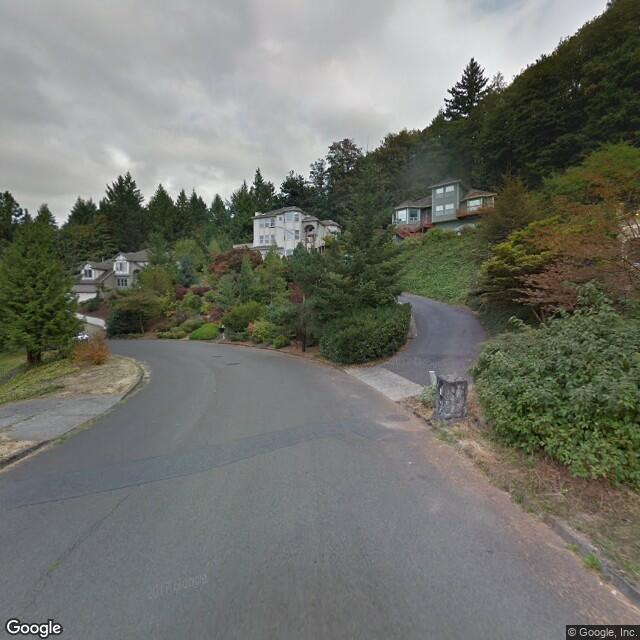
\includegraphics[width=0.25\linewidth]{input.jpg}
	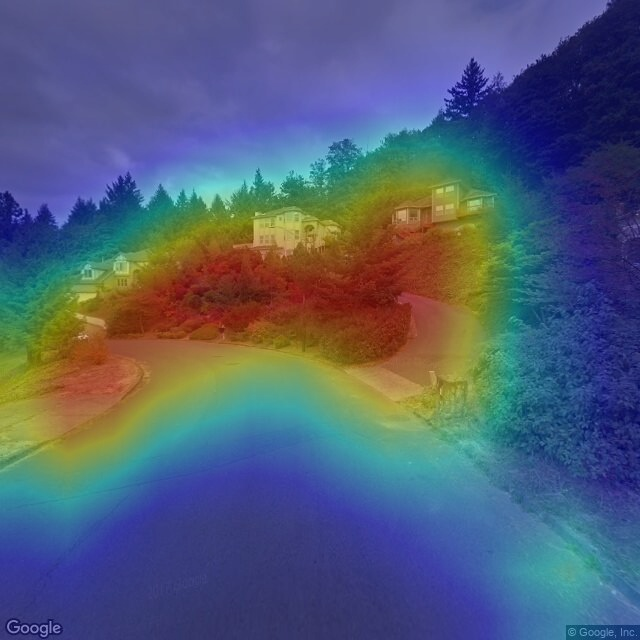
\includegraphics[width=0.25\linewidth]{cam.jpg}
	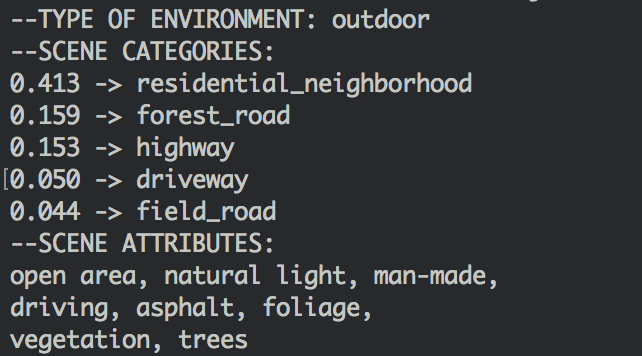
\includegraphics[width=.45\linewidth]{classification.png}
}
   
\end{center}
   \caption{Input image, class activation map, and predicted scene categories and attributes from Places365-ResNet50.}
\label{fig:short}
\end{figure*}

\subsection{Evaluation}

We expect our classifier to be able to classify unseen street-view images as bike-friendly or not with precision and recall better than a naive guess. We will train the classifier on 80\% of our dataset and evaluate it on the remaining 20\%. Additionally, we expect our inner layers to identify useful and sensible features; for example, we expect that images of bike-friendly streets are more likely to contain cyclists in them.

%-------------------------------------------------------------------------
\section{Technical Approach}

Our classifier will extend a pre-trained Places365-ResNet50 model. Created by MIT CSAIL, Places365 is a scene classifier based on the Places365 dataset, which contains millions of scene images labeled with 365 semantic categories and additional image attributes. For example, for each image the Places365 classifier predicts: 

\begin{itemize}
	\item scene classification ("residential\_neighborhood", "kitchen", "restaurant")
	\item attributes ("trees", "asphalt", "natural\_light")
	\item class activation maps
\end{itemize}

We will employ transfer learning to adapt the pre-trained Places365-ResNet50 model to the bike-friendly road classification task, and train the network on our labeled street-view images dataset.

%-------------------------------------------------------------------------
\section{Preliminary Results}

\subsection{Data}

We have developed scripts to generate our labeled dataset, and used it to create a sample dataset of 1000 images from streets in Portland, Oregon. We determined that \_ percent of the downloaded images are high-quality: they are correctly labeled, oriented in the right direction, and do not contain blur or other image artifacts. 

We have identified additional cities that are bike-friendly, have high quality OpenStreetMap data, and are almost entirely captured by Google Street View. Such cities include, but are not limited to: Pittsburgh, Boulder, Chicago, Washington DC, Seattle, Madison, and San Francisco. We aim to download at least 25,000 labeled images from these cities.

\subsection{Classifier}

We have set up the pre-trained Places365-ResNet50 network in a Google Cloud virtual environment and predicted scene classification and attributes of images in our labeled dataset. The results of the tests are very promising: the classifier is able to identify subtle scene categories and attributes that we expect will be valuable for our binary-classification task.

{\small
\bibliographystyle{ieee}
\bibliography{egbib}
}

\end{document}
